%%
%% This is file `tikzposter-example.tex',
%% generated with the docstrip utility.
%%
%% The original source files were:
%%
%% tikzposter.dtx  (with options: `tikzposter-example.tex')
%% 
%% This is a generated file.
%% 
%% Copyright (C) 2014 by Pascal Richter, Elena Botoeva, Richard Barnard, and Dirk Surmann
%% 
%% This file may be distributed and/or modified under the
%% conditions of the LaTeX Project Public License, either
%% version 2.0 of this license or (at your option) any later
%% version. The latest version of this license is in:
%% 
%% http://www.latex-project.org/lppl.txt
%% 
%% and version 2.0 or later is part of all distributions of
%% LaTeX version 2013/12/01 or later.
%% 








 \documentclass[25pt, a0paper, portrait, margin=0mm, innermargin=15mm,
     blockverticalspace=15mm, colspace=15mm, subcolspace=8mm]{tikzposter} %Default values for poster format options.

 \tikzposterlatexaffectionproofon %shows small comment on how the poster was made at bottom of poster

 % Commands
 \newcommand{\bs}{\textbackslash}   % backslash
 \newcommand{\cmd}[1]{{\bf \color{red}#1}}   % highlights command

 % Title, Author, Institute
 \title{Using tikzposter}
 \author{Pascal Richter, Elena Botoeva, Richard Barnard, \& Dirk Surmann}
 \institute{}

 % -- PREDEFINED THEMES ---------------------- %
 % Choose LAYOUT:  Default, Basic, Rays, Simple, Envelope, Wave, Board, Autumn, Desert,
 \usetheme{Autumn}
\usecolorstyle[colorPalette=BrownBlueOrange]{Germany}


 \begin{document}

     \maketitle

     \begin{columns}%blocks will be placed into columns
         \column{.55}
         \block[roundedcorners=40]{Creating the document}{
             The document begins with:
             \begin{quote}
                 \texttt{\bs documentclass[25pt, a0paper, portrait, margin=10mm, innermargin=15mm,
                 blockverticalspace=15mm, colspace=15mm, subcolspace=8mm]\{tikzposter\}\\
                 \bs title\{Title\}\\
                 \bs author\{Author(s)\}\\
                 \bs institute\{Institute \}\\
                 \bs titlegraphic\{Logo\}\\
                 \bs begin\{document\}\\
                 \bs maketitle}
             \\ \dots         \end{quote}

         \begin{tikzfigure}[A figure can be made with \bs \texttt{tikzfigure}; \bs\texttt{figure} does not work]
      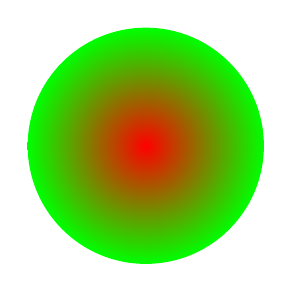
\begin{tikzpicture}
        \draw[draw=none,inner color=red, outer color=green] (0,0) circle (1.5cm);
      \end{tikzpicture}
         \end{tikzfigure}
 \innerblock[]{Inner Blocks}{Inner blocks may be created inside of blocks with the command \bs\texttt{innerblock[{\it options}]\{{\it Heading}\}\{{\it Text}\}} }
            \coloredbox{Text may be highlighted using colored boxes created by \bs\texttt{coloredbox[{\it options}]\{{\it Text\}}}}

     }
     \note[targetoffsetx=-.05\textwidth,targetoffsety=9.5cm,innersep=.4cm,angle=-45,connection]{Optional arguments for the format of the poster}
     \block{The title matter}{
         The title is made by the standard \texttt{\bs maketitle[{\it options}]} command where you can alter the \texttt{width}, the spacing between the title and top of the poster (\texttt{titletotopverticalspace}), the bottom of the title to the main content of the poster (\texttt{titletoblockverticalspace}) and the space between the title information and the logo (\texttt{titlegraphictotitleverticalspace}).

         If the default format of the title is not to your liking, you can define the placement of the different items via the \texttt{\bs settitle} command, described in the manual.
     }
     \block{Blocks}{
         Blocks are arranged in a grid, by default, with width by default \texttt{\bs textwdith}.  They are created by the command
         \begin{quote}
             \bs\texttt{block [{\it options}] \{{\it title}\}\{{\it contents}\}}
         \end{quote}
         The title may be left empty, resulting in no title area being created for the block (as seen in a later block to the right).  Further blocks will be placed below automatically, at a distance defined by \texttt{blockverticalspace}.

         If you want to change the position of the title matter or the contents in the block, you may by setting in the options
         \begin{quote}
             \texttt{titleoffsetx, titleoffsety, bodyoffsetx, bodyoffsety}
         \end{quote}
         which let you adjust the vertical or horizontal position of the two parts of the block, respectively.  You can also make, relative to the default width, the title and block body by setting
         \begin{quote}
             \texttt{titlewidthscale, bodywidthscale}
         \end{quote}
         The title's alignment can be set by \texttt{titleleft, titlecenter, titleright}, the body may be shifted vertically by setting \texttt{bodyverticalshift}, and the shape of the block can be altered by setting \texttt{roundedcorners, linewidth}. The inner margins of the title can by set by \texttt{titleinnersep,bodyinnersep}.
     }

     \note[targetoffsetx=24cm, targetoffsety=-9cm,rotate=1,angle=270,radius=8cm,width=.75\textwidth,innersep=.4cm]{
         You can place notes that are ``attached'' to the previous block using the command
         \begin{quote} \texttt{\bs note[{\it options}]\{{\it contents}\}}\end{quote}
         The note is placed by default slightly to the right of a ``target'' in the center of the previous block.  The note style may also allow for a connection between the note and the ``target''.  \\
         The target may be shifted from the default by setting the options  \texttt{targetoffsetx, targetoffsety}, rotated by an angle with \texttt{rotate}, and its width with \texttt{width}.  The placement of the note in relation with the target is given in polar coordinates with \texttt{ radius, angle}. Please observe that notes are always drawn {\bf over} the other objects. They do not affect the placement of blocks.
      }

     \column{.45}
         \block{Columns}{
              By default, blocks are arranged in a single column. If you want multiple columns for your poster, you may use the \texttt{columns} environment. For example,
             \begin{quote}
                 \texttt{\noindent \bs begin\{columns\}\\
                 \bs column\{.6\}\\
                 \bs block\{\dots\}\{\dots\}\\
                 \bs column\{.4\}\\
                 \bs block\{\dots\}\{\dots\}\\
                 \bs block\{\dots\}\{\dots\}\\
                 \bs end\{columns\}
                 }
             \end{quote}
             will create two columns of 60\% and 40\% the available width; spacing between successive columns is handled automatically.  The block command(s) following \texttt{\bs column} are the blocks to go in that column.  The number of columns is free to be chosen, but the relative widths must all be chosen.  If the widths sum to less than 1, empty space will be seen on the right.  If they sum to more than 1, the latter columns will be cut off.
         }

         \begin{subcolumns}
             \subcolumn{.45}
             \block{Subcolumns}{If you want to have an additional subdivision of columns inside a column, you may use the\\ \texttt{\bs subcolumns} environment inside of a column environment.  The functionality is similar to that of columns, but now the widths are relative to the width of the current column.}

             \subcolumn{.5}
             \block{}{An example use of subcolumns is.
                 \begin{quote}
                     \texttt{\bs begin\{subcolumns\}\\
                     \bs subcolumn\{.6\}\\
                     \bs block\{\dots\}\{\dots\}\\
                     \bs subcolumn\{.4\}\\
                     \bs block\{\dots\}\{\dots\}\\
                     \bs block\{\dots\}\{\dots\}\\
                     \bs end\{subcolumns\}
                     }
             \end{quote}
         }
         \end{subcolumns}

         \block[titlewidthscale=.8,bodywidthscale=.9,titleoffsety=9.5mm,bodyoffsety=9mm]{Changing the Poster's Appearance}{
             If the default appearance of the title, background, blocks, and notes is not desired, you may change the colors by calling the color style along with a general layout theme with the commands
             \begin{quote}
       \texttt{\bs usecolorpalette}\{{\em color palette}\}\\
                 \texttt{\bs usecolorstyle\{{\em color style}\}}
             \end{quote}
             and
             \begin{quote}
                 \texttt{\bs usetheme\{{\em layout style}\}}
             \end{quote}
             where the color palette and style and layout style are either the name of a custom made or one of the offered predefined choices listed in the manual or the comments of this poster's source.  Individual changes can be made to the style of the  background, title matter, blocks, inner blocks, and notes by using one of the following (along with either a custom-designed style or a predefined style listed in the manual or the comments of this poster's source).  These changes are made with the commands
             \begin{quote}
                 \texttt{\bs usebackgroundstyle[]\{\}, \bs usetitlestyle[]\{\},\\ \bs useblockstyle[]\{\},\bs innerblockstyle[]\{\}, \bs usenotestyle[]\{\}}
             \end{quote}
             Custom styles for these can be made; this is detailed in the manual.
          }

     \end{columns}

     \block[titleoffsety=-1cm,bodyoffsety=-1cm]{Sample document}{\vspace{2em}
         This poster was created by the following commands (omitting the contents of the blocks and notes) to give a sense of how different objects are created and options used.
         \begin{quote}
             \texttt{\bs documentclass[25pt, a0paper, portrait, margin=0mm, innermargin=15mm,
         blockverticalspace=15mm, colspace=15mm, subcolspace=8mm]\{tikzposter\}\\
             \bs title\{Using tikzposter\} \bs author\{Pascal Richter, Elena Botoeva, Richard Barnard, \& Dirk Surmann\} \bs institute\{\}\\
              \bs usetheme\{Autumn\}\bs usecolorstyle[colorPalette=BrownBlueOrange]\{Germany\}\\
             \bs begin\{document\}\bs maketitle\\
             \bs begin\{columns\} \bs column\{0.55\}\\
             \bs block\{Creating the document\}\{The document\dots\} \bs note[targetoffsetx=-.05\bs textwidth,targetoffsety=9.5cm,innersep=.4cm,angle=-45,connection]\{\dots\}\\
             \bs block\{The title matter\}\{The title\dots\}\\
             \bs block\{Blocks\}\{Blocks are\dots\} \bs note[targetoffsetx=24cm, targetoffsety=-9cm,rotate=1,angle=270,radius=8cm,width=.75\bs textwidth,innersep=.4cm]\{You can\dots\}\\
             \bs column\{0.45\} \bs block\{Columns\}\{By default,\dots\}\\
             \bs begin\{subcolumns\} \bs subcolumn\{.45\}
             \bs block\{Subcolumns\}\{If you\dots\}
             \bs subcolumn\{.5\} \bs block\{\}\{An example\dots\}
             \bs end\{subcolumns\}\\
             \bs block[titlewidthscale=.8,bodywidthscale=.9,titleoffsety=9.5mm,bodyoffsety=9mm]\{Changing the Poster's Appearance\}\{If the default\dots\}
             \bs end\{columns\}\\
             \bs block[titleoffsety=-1cm,bodyoffsety=-1cm]\{Sample document\}\{This poster\dots\}\\
             \bs end\{document\}
             }
         \end{quote}
     }

 \end{document}




\endinput
%%
%% End of file `tikzposter-example.tex'.
